\addcontentsline{toc}{section}{Introduction}
\section*{Introduction}
Nous abordons, dans ce chapitre, la présentation de la méthodologie et des choix techniques. Nous voulons mettre en place un modèle de reconnaissance vocal. Ce model sera des réseaux de neurones profonde (DNN). Nous avons vu précédemment qu’il existait plusieurs méthodes de Deep Learning pour la reconnaissance par empreinte vocale. Dans ce chapitre, nous allons effectuer un choix et approfondir la méthode choisie. Nous allons commencer par la méthode de Deep Learning choisie et l’architecture du système que nous voulons mettre en place. Nous aborderons également les matériels ainsi que les technologies utilisées dans la mise en œuvre du modèle. 

\section{Architecture du système}
La finalité de ce travail est de mettre en place un modèle d’IA pour identification et l’authentification par empreinte vocale. L’IA sera ensuite déployée comme un cloud REST API pour permettre à divers client web ou mobile de pouvoir y accéder.  Ainsi l’architecture sera composée de trois parties : 
\begin{enumerate}
    \item le code de paramétrage de l’IA et la gestion du dataset
    \item Le notebook Google Colab pour l’entrainement 
    \item la partie backend pour servir les APIs d’identification et d’authentification. 
\end{enumerate}
Chacune de ces partie joue un rôle spécifique : 
\begin{itemize}
    \item la partie 1 permet de gérer les paramètres d’exécution et gère l’entrainement du model. 
    \item Le notebook va nous permettre de préparer nos données d’entrainer le model, d’effectuer l’inférence et d’exporter le model optimal vers le backend pour servir le cloud API. 
    \item la partie backend va mettre en œuvre un projet Django qui va offrir les différents API d’identification et d’authentification entre autre. 
\end{itemize}

\section{Matériels}
Le code d’entrainement sera exécuté sur Colab qui nous offre une machine linux avec toutes les ressources CPU, GPU nécessaire a une telle opération. 

\begin{figure}[ht]
    \begin{center}
        \centering
        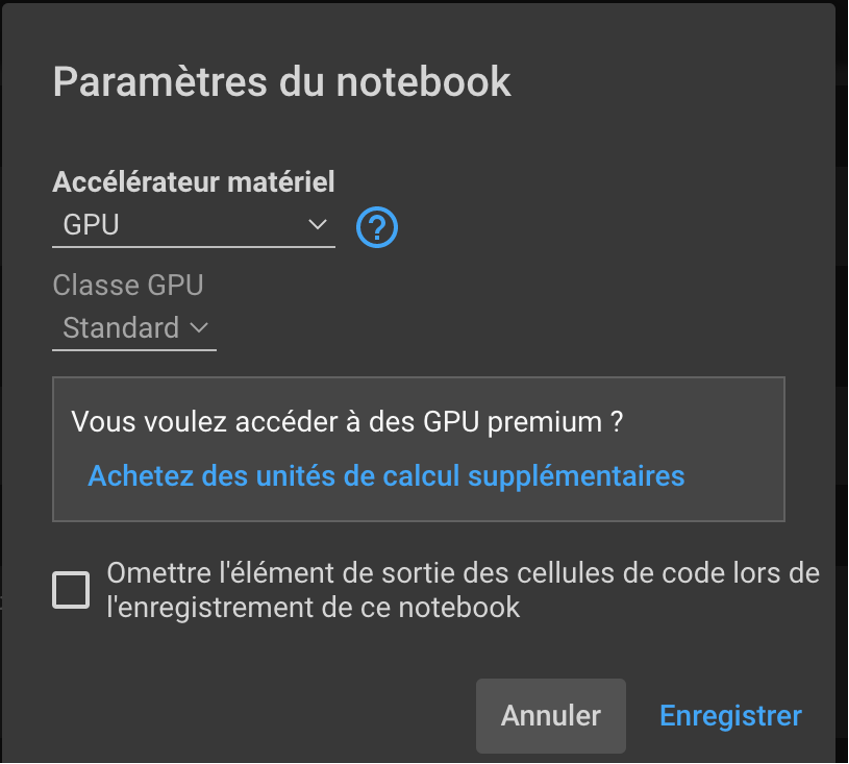
\includegraphics[width=1\textwidth]{2-clab-1}
        \caption{paramètres d'exécution du Colab}
        \label{fig:2-clab-1}
    
    \end{center}
\end{figure}


\begin{figure}
    \begin{center}
        \centering
        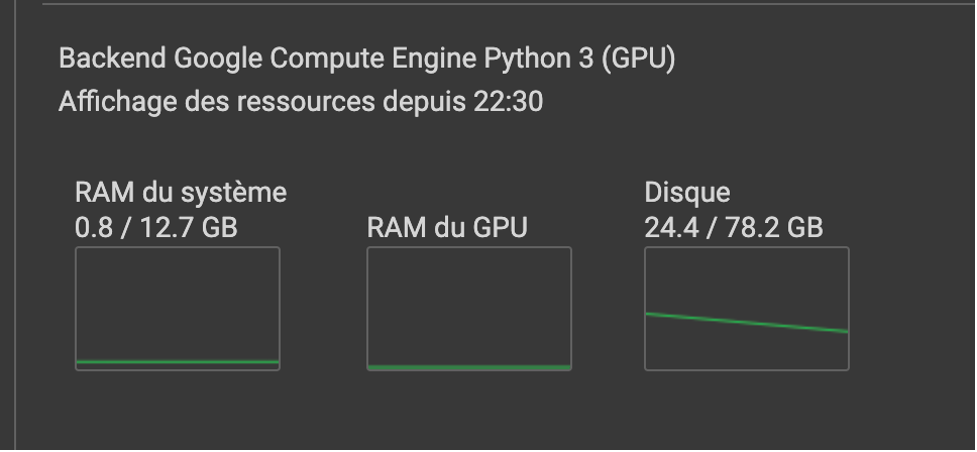
\includegraphics[width=1\textwidth]{2-clab-2}
        \caption{Ressource de l'environnement d'exécution Colab}
        \label{fig:2-clab-2}
        
    \end{center}
\end{figure}




\paragraph{}Le data-set sera sauvegardé sur Google Cloud Storage. En ce qui concerne le backend il sera déployé sur un backend sur le cloud. 

\section{Choix technologique}
\subsection{Définitions }
\paragraph{}\textbf{La reconnaissance de locuteurs}  est utilisée dans de nombreux domaines, tels que la sécurité, la biométrie, la communication et l'analyse de données. Pour réaliser cette reconnaissance, plusieurs méthodes peuvent être utilisées, notamment la reconnaissance automatique de la parole, l'analyse acoustique, la modélisation de la voix et l'apprentissage automatique.
\paragraph{}\textbf{Les x-vectors} sont des vecteurs d'embedding de haut niveau extraits à partir de caractéristiques acoustiques et utilisés pour la reconnaissance automatique de la parole et la vérification du locuteur. Pour extraire les x-vectors, un modèle de réseau de neurones à décalage temporel (TDNN) est souvent utilisé.
Le modèle TDNN pour les x-vectors est entraîné sur de grandes quantités de données de parole pour apprendre à extraire les caractéristiques acoustiques les plus discriminantes pour la reconnaissance du locuteur. Le modèle est ensuite utilisé pour extraire les x-vectors des enregistrements de parole et ces vecteurs sont utilisés pour identifier les locuteurs ou vérifier leur identité.
Nous avons vu dans le chapitre premier que plusieurs méthodes de deep learning pouvaient permettre d’entrainer des modèles de reconnaissance de locuteurs.  Dans le cas de notre étude nous utiliserons les TDNN.
\paragraph{}\textbf{Le TDNN (Time-Delay Neural Networkest)} est une méthode de traitement de la parole qui se concentre sur les caractéristiques temporelles de la parole plutôt que sur les caractéristiques fréquentielles.
Le TDNN utilise une fenêtre temporelle glissante pour extraire des caractéristiques de la parole à partir de segments de durée fixe. Ces caractéristiques sont ensuite traitées par des couches de neurones, chaque couche traitant des caractéristiques de plus en plus abstraites. Le TDNN utilise également des couches de rétropropagation de l'erreur pour ajuster les poids des neurones en fonction de l'erreur de prédiction.
Le TDNN est particulièrement utile pour la reconnaissance de locuteur car il est capable de traiter \textbf{les variations temporelles de la parole, telles que les pauses, les changements de ton et les variations de vitesse. Il peut également être utilisé pour détecter les caractéristiques distinctives de la voix d'un locuteur, telles que la hauteur, la durée et le débit de la parole.}
\paragraph{}\textbf{Le TDNN} est également un type de réseau de neurones convolutif (CNN) qui prend en compte les caractéristiques temporelles dans les données d'entrée. Il utilise des convolutions sur des fenêtres de temps pour extraire des caractéristiques pertinentes de la parole. Le TDNN est ensuite suivi d'une couche d'agrégation globale pour résumer les caractéristiques de la parole dans un vecteur d'embedding de haut niveau (X-Vector).

\paragraph{}En résumé, le TDNN est un outil puissant pour la reconnaissance de locuteur car il peut prendre en compte les informations temporelles de la parole et les variations de la parole dues aux différences de prononciation et de dialecte. Il peut être entraîné à reconnaître les locuteurs à partir d'enregistrements vocaux et peut être utilisé pour prédire le locuteur d'un enregistrement vocal inconnu.

\subsection{Structure }
Les TDNN sont constitués  d'une couche d'entrée, de plusieurs couches cachées et d'une couches de sortie mais ils se différencie de par l'organisation des liaisons inter-couches. Les TDNN introduisent des contraintes qui leurs permettent d'avoir un certain degré d'invariance par décalage temporel et déformation. Celles-ci utilisent trois idées : poids partagés, fenêtre temporelle et délai.
Les poids partagés permettent de réduire le nombre de paramètres du réseau neuronal et induisent ainsi une capacité de généralisation plus importante. Les poids sont partagés suivant la direction temporelle, c'est à dire que pour une caractéristique donnée, la fenêtre associée à celle-ci aura les mêmes poids selon la direction temporelle. De plus cette contrainte entraîne une capacité d'extraire les différences au fur et à mesure du balayage du signal. 
Le concept de fenêtre temporelle implique que chaque neurone de la couche l+1 n'est connecté qu'à un sous ensemble de la couche l (nous n'avons plus une connectivité totale). La taille de cette fenêtre est la même entre deux couches données. Cette fenêtre temporelle permet que chaque neurone n'est qu'une vision locale du signal, il peut être vu comme une unité de détection d'une caractéristique locale du signal.
En plus des deux contraintes précédente nous introduisons des délais entre deux fenêtre successive pour une couche donnée.
De plus chaque couche a deux directions : une direction temporelle et une direction caractéristique \cite{frontiers}.

\begin{figure}[ht]
    \centering
    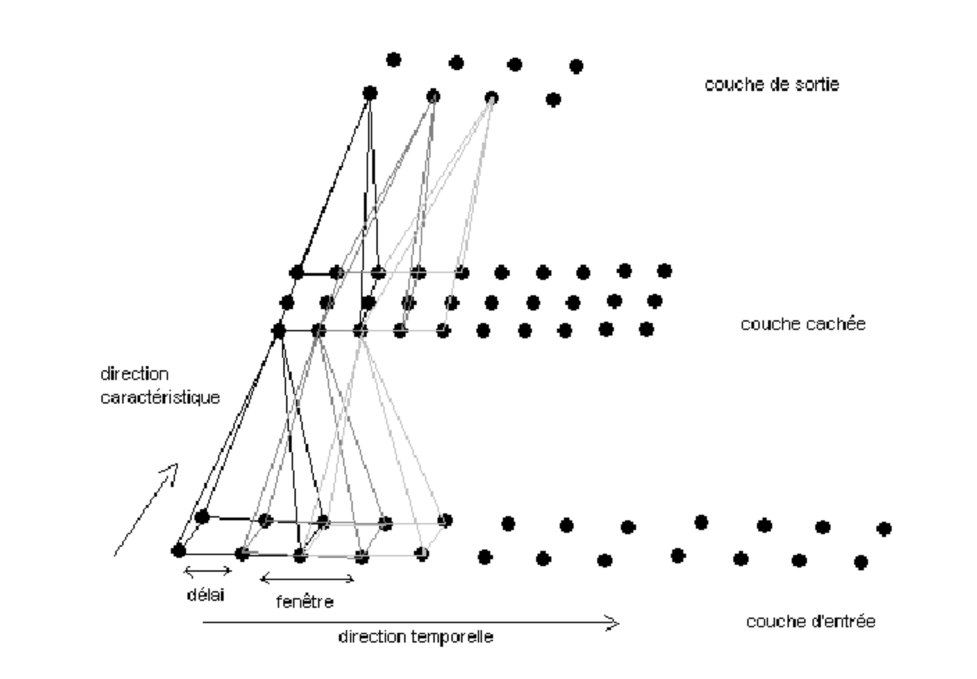
\includegraphics[width=1\textwidth]{2-clab-3}
    \caption{Structure d'un RN de type TDNN}
    % \captionsource{Caption}{ref, cite or free Text}
    \source{The Marvin Project}
    \label{fig:2-clab-3}
\end{figure}

\subsection{Fonctionnement }

\paragraph{}Le but du TDNN est non pas d'apprendre basiquement le signal mais d'extraire les caractéristique de celui-ci. La première couche acquière le signal puis une ou plusieurs couches cachées transforment le signal en des vecteurs de caractéristiques(X-Vectors). Un neurone donné détecte une caractéristique locale de la variation de la courbe. Le champ de vision du neurone est restreint à une fenêtre temporelle limitée. Avec la contrainte des poids partagés, le même neurone est dupliqué dans la direction temps (la même matrice de poids dupliquée) pour détecter la présence ou l'absence de la même caractéristique à différentes places le long du signal. En utilisant plusieurs neurones à chaque position temporelle, le réseau de neurone effectue la détection de caractéristiques différentes : les sorties des différents neurones produisent un nouveau vecteur caractéristique pour la couche supérieure.
\paragraph{}La composante temporelle du signal d'origine est peu à peu éliminée au fur et à mesure de sa transformation en caractéristique par les couches supérieures, pour compenser cette perte d'information on augmente le nombre de neurones dans la direction caractéristique \cite{themarvinproject}.


\addcontentsline{toc}{section}{Conclusion}
\section*{Conclusion}
\paragraph{}Dans ce chapitre, nous avons présenté l’architecture de notre système, les matériels ainsi que les différentes technologies utilisées dans le cadre de notre travail. En ce qui concerne le choix de la méthodologie nous avons opté pour le TDNN. 
\paragraph{}Il faut retenir que le TDNN (Time Delay Neural Network) est une technique d'apprentissage profond qui est largement utilisée pour la reconnaissance de locuteurs. Cette méthode a l'avantage de traiter les signaux acoustiques dans leur temporalité, ce qui permet de prendre en compte les variations temporelles des caractéristiques acoustiques des locuteurs. Le TDNN est également capable de traiter des données de haute dimensionnalité, telles que les signaux audios, en utilisant des réseaux de neurones profonds, ce qui en fait une méthode performante pour la reconnaissance de locuteurs. Dans notre implémentation, il nous permettra d’extraire les x-vectors à partir des caractéristiques acoustiques afin de faire l’identification ou l’authentification du locuteur.
